\subsection{Curves and Point Arithmetic}
\label{sec:math_curve}

As point multiplication is the action that takes the most time to perform,\cite{safecurves} several algorithms exist to
speed this up. Some of these will be discussed here (Section \ref{sec:math_curve_multiplication}). While only Weierstrass
curves are discussed in detail, the differences between Weierstrass curves and curves of other forms are touched upon briefly
(Section \ref{sec:math_curve_curves}).

Conceptually, the addition of two points, \(P + Q = R\), is done by drawing a line through the points, \(P\) and \(Q\),
and finding the point \(-R\), where the line intersects the curve again. This point is
then reflected over the x-axis to find \(R\), the result.

\begin{figure}[htb]
	\centering
	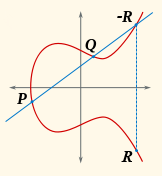
\includegraphics{maths/addition}
	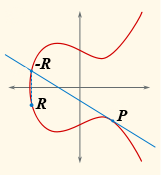
\includegraphics{maths/doubling}
	\caption{Conceptual addition (left) and doubling (right) of points on elliptic curves.}
\end{figure}

There are a few cases that are not explained by this conceptual model: if a point is added to its reflection, \(P + (-P)\),
the line drawn through the two points will not intersect the curve at any other point. The result of such an addition is
the point at infinity, \(O_\infty\). An addition where one point is the point at infinity will be the point that is not
infinity: \(P + O_\infty = P\).

The double of \(P\), \(2P\) or \(P+P\), is found by drawing the tangent of the curve at \(P\).
\(-R\) is once again found at the line's (in this case the tangent's) next intersection
with the curve, and the result \(R\), is found by reflecting \(-R\).\cite{hankerson2010}

\subsubsection{Weierstrass Curves}

Weierstrass simple form is very easy to perform operations on. This is also the one
BouncyCastle primarily supports (\verb|FpCurve|). Weierstrass curves are of the form
\(y^2 = x^3 + ax + b\). Arithmetic operations on points in a curve of the Weierstrass
simple form are fairly easy to implement.
\paragraph{Addition}

Addition of two points \(P + Q = R\) is a fairly straight-forward matter. Given two points, \(P = (x_1,y_1)\) and
\(Q = (x_2,y_2)\), the result \(R = (x_3,y_3)\) can be found with the following calculations:

\begin{equation}
	\lambda = {{y_2-y_1} \over {x_2-x_1}}
\end{equation}

\begin{equation}
	x_3 = \lambda^2 - x_1 - x_2 \textbf{ and } y_3 = \lambda (x_1 - x_3) - y_1
\end{equation}

As elliptic curves also contain the \(\infty\) (infinity) point, there is a single exception to this
rule: if either \(P\) or \(Q\) is infinity, the result of adding them will be infinity, too.

\begin{equation}
    Q = \infty \lor P = \infty \implies P + Q = \infty\
\end{equation}

\paragraph{Doubling}

If the points being added are equal to one another (\(P + Q = R \text{, where } P = Q \text{ and } P = (x_1,y_1)\)),
the result can be calculated with a simplified formula:

\begin{equation}
	\lambda = {{3x_1^2 + a} \over {2y_1}} \text{, where } a \text { is the parameter from the curve formula }
\end{equation}

\begin{equation}
	x_3 = \lambda^2 - 2x_1 \textbf{ and } y_3 = \lambda (x_1 - x_3) - y_1
\end{equation}

The resulting point is then \(R = (x_3, y_3)\).

\paragraph{Subtraction}

A subtraction \(P - Q = R\) can be expressed through addition and negation, as \(P - Q = P + (-Q)\). Negation of a given point
\(P = (x,y)\) is calculated as \(-P = (x,-y)\) (a reflection over the x-axis).

As with addition, negation is complicated by the existence of the infinity point:

\begin{equation}
	-\infty = \infty \textbf{ and } P - P = \infty
\end{equation}

The negation of infinity is infinity (negative infinity does not exist), and a point subtracted from itself is infinity.\cite{hankerson2010}

\subsubsection{Scalar Multiplication}

Scalar multiplication of a point \(P\) and an integer \(d\) is, with the most simple algorithm, calculated through repeated addition
of the point to an accumulator. Several algorithms to speed up this process exist, and as point multiplication is most computational
time is spent\footnote{See Section \ref{sec:performance_components} for a confirmation of this.} a few are covered in the following:
\emph{Double-and-Add}, \emph{NAF}, and \emph{wNAF}.

\paragraph{Double-and-Add}

The DoubleAndAdd method limits the number of additions necessary by doubling the accumulating result whenever possible, resulting in
fewer total additions.

The algorithm relies on first representing the number \(d\) in its binary form, \(d_{binary} = (d_{t-1}, ... , d_2, d_1, d_0)_2\),
where \(t\) is the number of bits used to represent the number. Each bit is then inspected, from least significant (right) to most
significant (left): if the bit is \(1\), the current value of \(P\) is added to the accumulator. For each bit inspected, \(P\) is
doubled.\cite{hankerson2010}

This algorithm results in \(~1.5t\) additions (most of which are doublings), much less than the \(~0.5t^2\) additions required for
repeatedly adding the point to an accumulator.

\paragraph{Non-adjacent form}

Whereas the binary form of a number is constructed from \(\{0,1\}\), the non-adjacent form (NAF) is constructed from \(\{-1,0,1\}\), with
the added limitation that no non-zero values are adjacent (hence the name). Subtraction of points is (almost) as efficient as addition,
requiring only an additional negation of a finite field element (see above).

The NAF of a number \(d\) can be constructed by an algorithm, which finds each digit as \(d_i = 2 - (d \text{ mod } 4)\) if \(d\) is odd, and
\(0\) otherwise. \(d\) is then reduced by \(d_i\) and halved, before the algorithm repeats for the next value. This continues until \(d < 1\).

The multiplication \(dP\) can be calculated using the \(NAF(d)\) with an appropriate algorithm (see Figure \ref{fig:naf-algorithm}).\cite{hankerson2010}

\begin{figure}[htb!]
	\centering
	\begin{tabular}{|p{\textwidth}|}
		\hline
		Input: Positive integer \(k\), \(P \in E(\mathbb{F}_q)\). \\
		Output: \(kP\).

		\begin{enumerate*}
			\item Compute \(NAF(k) = \Sigma^{l-1}_{i=0} k_i2^i\).
			\item \(Q \gets \infty\).
			\item For \(i\) from \(l-1\) downto \(0\) do
			\begin{enumerate*}
				\item \(Q \gets 2Q\).
				\item If \(k_i = 1\) then \(Q \gets Q + P\).
				\item If \(k_1 = -1\) then \(Q \gets Q - P\).
			\end{enumerate*}
			\item Return(\(Q\)).
		\end{enumerate*}
		\\
		\hline
	\end{tabular}
	\caption{The algorithm for computing the scalar multiplication \(kP\) using the non-adjacent form of \(k\), as represented by
		Hankerson et.al.\cite{hankerson2010}}
	\label{fig:naf-algorithm}
\end{figure}

The running time for the NAF algorithm is approximately \(1 {1 \over 3} l\), where \(l\) is the length of the NAF, quicker than that
of the Double-and-Add.\cite{hankerson2010}

\paragraph{Windowed NAF}

The NAF can be improved further by allowing a wider range of values than just those in \(\{-1,0,1\}\). The range is called a \emph{window}, and
using this windowed non-adjacent form (wNAF) can improve running time, but requires some pre-computation. Regular \(NAF\) is the same
as \(wNAF_2\) (a window size of 2), and \(wNAF_3\) would be constructed from the values \(\{-3,-1,0,1,3\}\).

The wNAF of an integer is calculated in much the same way as a NAF, but with some added complexity due to the variable size of \(w\)
(see Figure \ref{fig:compute-wnaf-algorithm}).

\begin{figure}[htb!]
	\begin{tabular}{|p{\textwidth}|}
		\hline
		Input: Window width \(w\), positive integer \(k\). \\
		Output: \(NAF_w(k)\).
		\begin{enumerate*}
			\item \(i \gets 0\).
			\item While \(k \geq 1\) do
			\begin{enumerate*}
				\item If \(k\) is odd then: \(k_i \gets k \text{ mods } 2^w\), \(k \gets k - k_i\);
				\item Else: \(k_i \gets 0\).
				\item \(k \gets k/2\), \(i \gets i + 1\).
			\end{enumerate*}
			\item Return(\(k_{i-1},k_{i-2},...,k_1,k_0\)).
		\end{enumerate*} \\
		\hline
		Where \(k \text{ mods } 2^w\) is: 
		\begin{enumerate*}
			\item If \(k \text{ mod } 2^w \geq 2^{w-1}\) then return(\((k \text{ mod } 2^w) - 2^w\));
			\item Else return(\(k \text{ mod } 2^w\)).
		\end{enumerate*} \\
		\hline
	\end{tabular}
	\caption{The algorithm for constructing a wNAF representation of an integer \(k\), as represented by Hankerson
		et.al.\cite{hankerson2010} Here with added explanation of \(k \text{ mods } 2^w\).}
	\label{fig:compute-wnaf-algorithm}
\end{figure}

The wNAF multiplication algorithm relies on the precomputation of the values \(P_i = iP \text{ for } i \in \{1,3,5,...,2^{w-1}-1\}\). If the
point \(P\) is fixed for many operations, then this precomputation may be worthwhile, even at big values for \(w\). For dynamically varying
\(P\) (such as in asymmetric encryption) a large \(w\) may result in an overhead larger than the benefit of the quicker operations.

The wNAF multiplication algorithm is very similar to that of the regular NAF, distinguishing itself by its precomputation and slightly more
advanced structure for non-zero \(k_i\) (see Figure \ref{fig:wnaf-algorithm}).

\begin{figure}[htb!]
	\begin{tabular}{|p{\textwidth}|}
		\hline
		Input: Window width \(w\), positive integer \(k\), \(P \in E(\mathbb{F}_q)\).\\
		Output: \(kP\).
		\begin{enumerate*}
			\item Compute \(wNAF_w(k) = \Sigma^{l-1}_{i=0} k_i 2^i\).
			\item Compute \(P_i = iP\) for \(i \in \{1,3,5,...,2^{w-1}-1\}\).
			\item \(Q \gets \infty\).
			\item For \(i\) from \(l - 1\) downto \(0\) do
			\begin{enumerate*}
				\item \(Q \gets 2Q\).
				\item If \(k_i \neq 0\) then:
				\begin{enumerate*}
					\item If \(k_i > 0\) then \(Q \gets Q + P_{k_i}\);
					\item Else \(Q \gets Q - P_{-k_i}\).
				\end{enumerate*}
			\end{enumerate*}
			\item Return(\(Q\)).
		\end{enumerate*} \\
		\hline
	\end{tabular}
	\caption{Algorithm for computing the multiplication \(kP\) using the wNAF algorithm, as represented by Hankerson et.al.\cite{hankerson2010}}
	\label{fig:wnaf-algorithm}
\end{figure}

wNAF is a generalization of NAF, and so the formula for running time of wNAF is a generalization of the running time for NAF. The number of
additions performed in wNAF depends on the window \(w\) and can be described as \(2^{w-2} + (1 + {1 \over {w + 1}}) l\), where \(l\) is the length
of the wNAF form.
\subsubsection{Other Curve Forms}

There are more efficient representations of elliptic curves than the simple
Weierstrass form. Both Edwards or Montgomery curves are more recent than the simple Weierstrass forms,
and have shown to have some desirable properties.\cite{safecurves}

Neither Montgomery nor Edwards curves are supported in OpenECC, but they can be converted to the
usable Weierstrass form. Montgomery curves have the following formula:

\begin{equation}
	y^2 = x^3 + ax^2 + x
\end{equation}

Whereas it is possible to represent all curves in Weierstrass simple forms, the same cannot be said for
the Montgomery form (or the Edwards form for that matter). It is, however, possible to
transform any of the safe Montgomery curves to the Weierstrass form.\cite{safecurves}

This does not come without a cost as the Weierstrass form of a Montgomery curve will have
very large integers as its parameters, compared to those in the original Montgomery form. For example,
the Montgomery curve, \verb|Curve25519| has the equation \(y^2 = x^3+486662x^2+x\), but
translated into the Weierstrass simple form, it will have an equation that does not fit on the width of
a normal A4 page:\footnote{See the full calculations and equation in Appendix \ref{app:montgomery_weierstrass}.}

\begin{equation}
	y^2 =
	x^3 +
	19298681539552699237261830834781317975544997444273427339909597334573241639236x +
	55751746669818908907645289078257140818241103727901012315294400837956729358436
\end{equation}

These large parameters make Montgomery curves infeasible to use, as multiplication would be very slow. As such,
it is discouraged to use curves that are not normally in the Weierstrass form.\footnote{Unless support for Montgomery
curves is implemented in the future, which is enabled by the extendable structure of OpenECC (see Section
\ref{sec:implementation_curves}).}